\documentclass[conference]{IEEEtran}
\usepackage{booktabs,graphicx,url,amsmath}
\begin{document}
\title{NyxChat: A Serverless, Post-Quantum-Hybrid, Delay-Tolerant Messenger for Disconnected Environments}
\author{\emph{Author names and affiliations to be completed by the maintainers (GitHub: harshitt13) \and  Draft prepared September 2026}}
\maketitle
\begin{abstract}Secure messengers such as Signal depend on servers for discovery, key distribution and store-and-forward delivery, and stop working when the network does. Bluetooth mesh messengers work without infrastructure but have repeatedly shipped with weak or absent authentication, no forward secrecy, and no protection against relays that read or re-address traffic. We present NyxChat, an open-source Android messenger that combines both worlds: a mutually authenticated hybrid handshake (X3DH-style X25519 agreement plus Kyber-768 encapsulation, Ed25519-signed), the Signal Double Ratchet for every pairwise conversation, Sender Keys for groups, and a transport-agnostic \emph{envelope} that is delivered identically over an encrypted TCP link on Wi-Fi, over a Bluetooth Low Energy (BLE) mesh with store-and-forward relaying, or from a persistent outbox once a path appears. Sessions to contacts that are not reachable are bootstrapped without any server from pinned identity keys, and concurrent initiations are resolved deterministically. All direct links are additionally encrypted so that message metadata never crosses the air in the clear; keys are pinned on first use, changes are refused until the user compares safety numbers, and a duress password opens a decoy profile with independent keys. We implemented NyxChat in 12.8 kLOC of Dart plus a native Kotlin BLE peripheral, covered the cryptographic core with 43 unit tests, and evaluated it with micro-benchmarks, wire-size measurements and a mobility simulation that drives the real router: Spray-and-Wait relaying delivers 72-98\% of messages across 10-80 nodes at 3-4\% of the transmission cost of epidemic flooding. We also report, as a case study, the defects found in the previous version of the same application, which illustrate how an unaudited mesh messenger can claim properties its code does not provide.\end{abstract}
\section{1. Introduction}
Messaging is the application people reach for first in an emergency, and it is also the one most tightly bound to infrastructure. Signal, WhatsApp and iMessage provide strong end-to-end encryption \cite{ref2,ref13,ref18} but need a server to find peers, to exchange pre-keys and to hold messages until the recipient comes online. When cellular service is congested or cut, as during natural disasters, large demonstrations or deliberate shutdowns, those applications fail together with the network.

Infrastructure-free messengers fill that gap by relaying messages between nearby phones over Bluetooth or Wi-Fi. Their security record, however, is poor. Bridgefy, promoted during the 2019-2020 Hong Kong protests, was shown to allow impersonation, message decryption by relays and user tracking \cite{ref6,ref7}. Several newer BLE mesh applications have launched with no identity authentication at all, adding one only after public critique. The recurring pattern is that the routing problem is solved first and the cryptographic protocol is bolted on, without tests, and with documentation that promises more than the code delivers.

NyxChat is our attempt to build the messenger these situations need, treating the cryptographic protocol as the product rather than a feature. It makes four design commitments:

\begin{itemize}
  \item \textbf{One end-to-end unit, many transports.} Every payload is sealed into an \emph{envelope} whose authentication binds the sender and recipient identities. The envelope is the same whether it is carried in a link-encrypted TCP frame, in a mesh packet relayed by strangers' phones, or held for days in an outbox. Relays cannot read, alter or re-address it.
  \item \textbf{Authenticated, hybrid post-quantum key agreement.} Every direct link starts with a signed handshake that combines four X25519 Diffie-Hellman values with a Kyber-768 encapsulation. Sessions to contacts that are currently unreachable are derived from pinned identity and Kyber keys with no server involvement.
  \item \textbf{Standard ratchets, implemented carefully.} Pairwise conversations use the Signal Double Ratchet \cite{ref2} with commit-on-success state handling and persisted sessions; groups use Sender Keys with per-message signatures and rotation on membership change.
  \item \textbf{Trust the user can inspect.} Keys are pinned on first contact, a change is refused until accepted, and 60-digit safety numbers and QR contact cards let users verify each other out of band.
\end{itemize}
The contributions of this paper are: (i) the design of a transport-agnostic secure messaging layer that unifies direct, mesh and store-and-forward delivery under one envelope format with a deterministic resolution of concurrent session initiation; (ii) a complete open-source implementation for Android, including a native BLE GATT server that gives Flutter applications a peripheral role; (iii) an evaluation of cryptographic cost, wire overhead and mesh delivery using the production router inside a mobility simulator; and (iv) a case study of the previous release of the same application, whose ratchet, handshake, post-quantum step and Bluetooth transport were all non-functional despite documentation to the contrary, with the lessons we drew for building such systems.

The rest of the paper is organised as follows. Section 2 reviews the protocols and systems we build on. Section 3 states the threat model. Sections 4 and 5 present the cryptographic design and the transport layer. Section 6 describes the implementation, Section 7 the evaluation and Section 8 the security analysis. Section 9 discusses limitations and future work, and Section 10 concludes.

\section{2. Background and Related Work}
\subsection{2.1 Secure messaging protocols}
The Signal protocol consists of X3DH \cite{ref1}, an asynchronous key agreement in which an initiator combines Diffie-Hellman values between its identity and ephemeral keys and the recipient's identity and pre-keys, and the Double Ratchet \cite{ref2}, which derives a fresh message key for every message from a root chain advanced by Diffie-Hellman ratchet steps and symmetric chains advanced by a key derivation function. The combination provides forward secrecy and post-compromise security; its formal analysis is given by Cohn-Gordon et al. \cite{ref3}. Signal's PQXDH \cite{ref4} and Apple's PQ3 \cite{ref18} add a post-quantum KEM (Kyber, standardised as ML-KEM in FIPS 203 \cite{ref5}) to the initial agreement so that recorded traffic cannot be decrypted by a future quantum computer. Group messaging in WhatsApp and Signal uses Sender Keys \cite{ref13}: each member distributes a symmetric chain and a signing key through pairwise sessions; Rösler et al. \cite{ref14} analysed the resulting group security and the importance of authenticated membership changes. Unger et al. \cite{ref23} survey the wider design space.

NyxChat adopts these designs rather than inventing new cryptography. What differs is the environment: there is no server to host pre-keys, so asynchronous agreement must use long-term keys the sender already holds; and there is no trusted transport, so the ratchet must tolerate out-of-order and duplicated delivery through relays.

\subsection{2.2 Delay-tolerant networking}
Delay-tolerant networking (DTN) \cite{ref10} addresses networks without a contemporaneous end-to-end path. Epidemic routing \cite{ref9} replicates every message to every encountered node and maximises delivery at the cost of bandwidth and storage. Spray-and-Wait \cite{ref8} bounds replication: the source sprays L copies, and holders wait until they meet the destination. NyxChat's router combines Spray-and-Wait with routes learned from the paths recorded in packets, so that a node with a known next hop forwards a single copy.

\subsection{2.3 Infrastructure-free messengers}
Briar \cite{ref11} routes messages over Bluetooth, Wi-Fi and Tor with its own Bramble transport protocol and pairwise handshakes; it targets contacts who have met in person and does not relay through strangers. Meshtastic \cite{ref12} uses LoRa radios for long-range text with channel keys rather than per-user identities. Bridgefy \cite{ref6} relayed through arbitrary phones but, as Albrecht et al. showed, its original protocol leaked social graphs, allowed message forgery and decryption by relays, and was vulnerable to a zip-bomb denial of service; Berty's Wesh \cite{ref20} pursues a similar goal with IPFS-based primitives. Several BLE mesh chat applications released in 2025 initially transmitted messages without any identity binding and added authenticated handshakes only after external review. NyxChat's contribution relative to these systems is the combination of relay-through-strangers delivery with a protocol that gives relays nothing to read or forge, and with the same forward-secret ratchet used for direct links.

\section{3. Threat Model}
We consider an application running on two or more Android devices that may be connected over a shared Wi-Fi network, directly reachable over BLE, or connected only through a chain of intermediate NyxChat devices that are not trusted. We assume the cryptographic primitives (X25519 \cite{ref17}, Ed25519 \cite{ref22}, AES-256-GCM, HKDF \cite{ref16}, Argon2id \cite{ref15}) are secure, and that Kyber-768 \cite{ref21} may or may not be; the design must remain secure if either the classical or the post-quantum component holds.

Adversaries and their capabilities:

\begin{itemize}
  \item \textbf{Passive observer} on the same Wi-Fi network or within Bluetooth range. Reads every byte transmitted.
  \item \textbf{Active network attacker} who can inject, modify, replay and drop traffic, including presenting itself as a peer during discovery.
  \item \textbf{Malicious relay}: a NyxChat device on the mesh path that runs modified software and may store, replay, alter or selectively drop packets, and colludes with other relays.
  \item \textbf{Device seizure}: physical access to a locked device, including a full disk image, with the ability to coerce the owner into entering a password.
  \item \textbf{Long-term key compromise} of one party at some point in time.
\end{itemize}
Security goals: confidentiality and integrity of message content and of in-conversation metadata (message ids, receipts, reactions, group membership) against all adversaries above; authentication of the peer's identity after first contact; forward secrecy and post-compromise security of conversations; unlinkability of transport-level metadata from a LAN observer beyond the fact that two devices communicate; confidentiality of data at rest under seizure, bounded by the password's entropy; and plausible deniability of the real profile under coercion.

Out of scope: malware on the endpoint, hardware side channels, denial of service by jamming, and a global adversary correlating traffic timing across the whole mesh. Mesh addressing uses stable hashes, so a relay can learn that two hashed identities communicate; we discuss this limitation in Section 8.

\section{4. Cryptographic Design}
\subsection{4.1 Identity}
Each device generates an X25519 identity key IK, an Ed25519 signing key SK and a Kyber-768 key KPK, and keeps the private halves in Android's keystore-backed secure storage. The user-visible handle is \texttt{NC-} followed by 64 bits of SHA-256 over a domain string and both classical public keys. Every peer re-derives the handle from the keys it is shown and refuses a handshake if they disagree, so a handle cannot be claimed without the corresponding keys. The handle is only a routing label; trust decisions use the full pinned keys (Section 4.9).

\subsection{4.2 Direct-link handshake}
When two devices connect over TCP they exchange one signed hello each. The initiator sends its identity, signing and Kyber public keys, an ephemeral X25519 key EK, a 128-bit nonce, its listening port and capability list; the responder answers with the same fields plus the initiator's nonce and a Kyber ciphertext computed against the initiator's KPK. Each hello is signed over a length-prefixed transcript of all its fields with the sender's Ed25519 key. Both sides then compute

dh1 = X25519(IK\_A, IK\_B), dh2 = X25519(EK\_A, IK\_B), dh3 = X25519(IK\_A, EK\_B), dh4 = X25519(EK\_A, EK\_B),

master = HKDF(salt = nonce\_A || nonce\_B, ikm = 0xFF\textasciicircum{}32 || dh1 || dh2 || dh3 || dh4 || kem, info = "NyxChat-Handshake-v3").

The structure is that of X3DH \cite{ref1} with the responder's ephemeral key playing the role of a signed pre-key, extended with the KEM secret as in PQXDH \cite{ref4}. dh1 authenticates both identity keys; dh2 and dh3 give forward secrecy against later compromise of either identity key; dh4 gives forward secrecy against compromise of both; the KEM secret protects recorded transcripts against a future quantum adversary. The responder's signature over the initiator's nonce prevents replay of a captured response, and the responder checks the initiator's keys against its pin store \emph{before} revealing its own hello, so a key-changed or impersonating initiator learns nothing beyond the refusal. Kyber is mandatory in protocol v3; there is no downgrade path.

From the master secret both sides derive two link keys (Section 4.3) and a ratchet root. The initiator is always the Double Ratchet's "Alice" with the responder's EK as the initial remote ratchet key, and sends a \emph{session-open} message immediately so the responder, who has no sending chain until it receives one message, can reply. If a session already exists from an earlier meeting it is kept; the new handshake only refreshes the link keys.

\subsection{4.3 Link layer}
After the handshake every frame on the link is sealed with AES-256-GCM under a per-direction key derived from the master secret, using a 64-bit counter as nonce and as associated data. The receiver requires the counter to equal the next expected value, so replayed, reordered or dropped-and-reinjected frames terminate the link. Everything above this layer, including pings, receipts, reactions, group updates and file chunks, is therefore hidden from a LAN observer, who sees two signed hellos followed by opaque lines. This is deliberately separate from end-to-end encryption: the link protects one hop against a local observer, the envelope protects the message against everyone on the path.

\subsection{4.4 Envelopes and inner messages}
An \emph{inner message} is a small JSON document with a type (text, file descriptor, reaction, receipt, sender-key distribution, group update, session-open), an id, a timestamp and a body. An \emph{envelope} wraps its ciphertext with the sender and recipient handles, the kind of encryption (pairwise ratchet or group sender key), the ratchet header, and optionally a session-init block (Section 4.6). The associated data of every envelope is a length-prefixed encoding of a domain string, the sender handle, the recipient handle and the kind, so a relay that changes any of them causes authentication to fail. Envelopes are what transports carry; the transports never see inner messages.

\subsection{4.5 Pairwise sessions}
Pairwise conversations use the Double Ratchet \cite{ref2} as specified: the root KDF is HKDF-SHA256 with the root key as salt and the DH output as input; the chain KDF derives the message key as HMAC(ck, 0x01) and the next chain key as HMAC(ck, 0x02); the message key is expanded by HKDF into an AES-256 key and a 96-bit nonce; and the header (ratchet public key, previous chain length, message number) is concatenated to the envelope's associated data. Up to 256 messages can be skipped per chain and 1024 skipped keys are retained, which is what allows delivery through relays that reorder or duplicate. Two implementation choices matter for robustness: every decrypt operates on a working copy of the state and commits only after the tag verifies, so a forged or corrupted envelope can never desynchronise a session; and sessions are serialised to the encrypted database after every step, so forward secrecy does not reset to identity-derived keys on every launch.

\subsection{4.6 Asynchronous sessions and collisions}
A user may write to a contact who is not connected. Without a server there is no pre-key bundle to fetch, but the sender holds the contact's pinned IK and KPK. The sender generates an ephemeral EK and computes dh1 = X25519(IK\_A, IK\_B), dh2 = X25519(EK\_A, IK\_B) and a Kyber encapsulation to KPK\_B; the ratchet root is HKDF over 0xFF\textasciicircum{}32 || dh1 || dh2 || kem. The recipient's identity key doubles as its initial ratchet key and is replaced by a fresh key at its first reply, after which the session is indistinguishable from one created by a handshake. The ephemeral key and Kyber ciphertext are attached to every envelope as a session-init block until the sender has decrypted a reply; a recipient that already accepted that block ignores repeats.

Two contacts may initiate towards each other before either message arrives. NyxChat resolves this deterministically: on receiving an init block while itself holding a pending initiation, the device with the lexicographically smaller handle ignores the incoming block, and the other adopts the incoming session, verified by decrypting the first message, and resends its own queued messages through it. If a device lost its session state (for example after a database reset) it fails to decrypt, and on a direct link both sides re-derive the session from the current handshake after a rate-limited \emph{session-reset} frame; messages that had been sent but not acknowledged as delivered are re-queued.

\subsection{4.7 Groups}
Each member owns, per group, a random 256-bit chain key and an Ed25519 signing key, distributed to the other members inside pairwise ratchet envelopes. A group message is encrypted with a key derived from the chain (HMAC step, HKDF expansion, AES-256-GCM with the envelope's associated data) and signed over the group id, iteration counter, ciphertext and associated data. Receivers verify the signature under the sender's distributed key before deriving message keys, retain up to 512 skipped keys for out-of-order delivery, and reject iterations they have already consumed. Membership updates travel through pairwise sessions and are accepted only from current members; whenever a member leaves or is removed, every remaining member rotates its chain and redistributes it, so the departed member cannot read later traffic, and receivers discard the departed member's chain.

\subsection{4.8 Files}
Ratcheting once per chunk would be wasteful and would make resumption awkward. Instead the sender hashes the file, generates a random 256-bit key and 64-bit nonce prefix, and sends a descriptor inside the ratchet. Each 32 KiB chunk is sealed with AES-256-GCM under nonce = prefix || chunk index and associated data (file id, index, total), so chunks verify independently, may arrive in any order, and a transfer can resume after a disconnect. The receiver writes chunks into a sparse temporary file and compares the SHA-256 of the result with the descriptor before exposing it.

\subsection{4.9 Trust management}
Keys are pinned on first contact. A later handshake presenting different keys for the same handle is refused, the user is told that the safety number changed, and the link stays blocked until they accept. A safety number is derived from both fingerprints by 5120 iterations of SHA-256, rendered as twelve groups of five digits; it is identical on both phones if no attacker is in the middle. A contact card, shown as a QR code and copyable as text, carries only public keys; importing one pins and marks the contact as verified without any network contact, which closes the trust-on-first-use window entirely for users who meet in person.

\subsection{4.10 Data at rest and coercion}
All local state, including ratchet sessions, sender keys, pinned keys and the outbox, lives in AES-256 encrypted database boxes under a random master key held in secure storage. With the optional lock, the master key is wrapped with AES-256-GCM under a key derived by Argon2id \cite{ref15} (32 MiB, two passes, two lanes); installations that used PBKDF2 are transparently re-wrapped on their next unlock. A duress password, verified through its own Argon2id hash, opens a second profile with independent identity keys and database boxes and may be configured to destroy the real profile first; five failed attempts wipe everything. Identity keys never enter the database, so a corrupted database is deleted and recreated without forcing re-onboarding.

\section{5. Transports and Delivery}
\subsection{5.1 Discovery and links}
On a shared network, devices advertise \texttt{\_nyxchat.\_tcp} through multicast DNS and dial each other; to avoid two simultaneous links between the same pair, the device with the smaller handle dials first and the other waits three seconds. If duplicate authenticated links still arise, both sides apply the same rule, keeping the link dialled by the smaller handle, so they never disagree about which link survives.

Over Bluetooth, standard Flutter libraries provide only the central role, which is why two instances of the previous version could never find each other. NyxChat ships a native Android GATT server that advertises the service UUID with the handle in the scan response and exposes a write characteristic for inbound chunks and a notify characteristic for outbound ones. Every device scans and advertises simultaneously, so a link can form in either role and one device may be central to some neighbours and peripheral to others. After a link forms, the handle is exchanged, the MTU is negotiated up to 512 bytes, and messages are chunked with a two-byte sequence and flag header.

\subsection{5.2 Mesh routing}
A mesh packet carries an envelope, a TTL of seven hops, a timestamp with 24-hour expiry, the SHA-256 hashes of the sender and recipient handles, and the list of relay hashes it has traversed. A node deduplicates by packet id, learns a route to the sender through the last relay listed, and delivers packets addressed to its own hash to the messaging layer. Packets for others are stored in a bounded queue and forwarded after a random delay of 0.2-2 seconds: to the learned next hop if one is known, otherwise as a spray of up to three copies among current neighbours. Whenever a new neighbour appears, up to three stored packets are offered to it, which is the "wait" phase of Spray-and-Wait \cite{ref8}. Periodic beacons with TTL 3 refresh routes. Because the payload is an envelope, a relay that reads, edits or re-addresses a packet gains nothing and causes only an authentication failure at the destination.

\subsection{5.3 Delivery state machine}
Sending a message tries three paths in order: the authenticated TCP link if the peer is connected, the mesh if the peer's keys are pinned and at least one BLE link is up, and otherwise the persistent outbox. The outbox stores inner messages in plaintext inside the encrypted database and re-encrypts them on every attempt, so a session reset never strands ciphertext; group messages, whose sender-key envelopes remain decryptable until the next rotation, are stored as envelopes. Attempts back off exponentially from five seconds to ten minutes and are reset whenever a session is established or a session-open arrives. Receivers acknowledge text and files with an end-to-end receipt inside the ratchet, which drives the sent, delivered and read states shown to the user and, for groups, the per-member delivery lists.

\subsection{5.4 Privacy controls}
Stealth mode stops all advertising, scanning and multicast announcements while keeping existing links; cover traffic sends random-sized packets to random hashes at random intervals so that idle and active periods look alike to a nearby observer; and a screenshot-blocking window flag, notification content control and disappearing messages complete the picture.

\section{6. Implementation}
NyxChat is written in Dart with Flutter for the user interface and a small Kotlin component for the BLE peripheral. Table 1 summarises the code base. Cryptographic primitives come from \texttt{package:cryptography} (X25519, Ed25519, HKDF, HMAC, AES-GCM, Argon2id) and Kyber-768 from \texttt{package:post\_quantum}, a pure-Dart implementation of the round-3 CRYSTALS-Kyber construction; the lattice arithmetic and Argon2id run on background isolates so that the interface stays responsive.

\begin{table}[t]\centering\footnotesize
\caption{Size of the NyxChat code base (protocol v3).}
\begin{tabular}{ll}\toprule
Component & Dart lines \\ \midrule
Cryptographic core and protocol formats (\texttt{core/crypto}, \texttt{core/protocol}) & 2,644 \\
Networking, mesh and storage (\texttt{core/network}, \texttt{core/mesh}, \texttt{core/storage}) & 3,692 \\
Services (identity, lock, settings, messaging engine, discovery) & 2,366 \\
User interface & 2,627 \\
Native Android BLE peripheral and window security (Kotlin) & 304 \\
Tests (43 unit tests, benchmark harness, mesh simulator) & 1,169 \\
\bottomrule\end{tabular}\end{table}
Several engineering details are security-relevant. Every parser enforces types, key lengths and size limits (1 MiB per link frame, 512 KiB per envelope, 64 KiB per mesh packet), and a socket that exceeds its buffer is closed. Frames on a link are processed strictly in order even though socket events arrive asynchronously, because link decryption is stateful. Secret buffers are zeroed after use where the runtime allows. The handshake, ratchet, sender keys, secure channel, session manager, trust store and outbox are exercised by 43 unit tests that include tampering, replay, out-of-order delivery across ratchet boundaries, forged signatures, nonce mismatch, key-change refusal, persistence round trips and the initiation-collision rule. Continuous integration runs analysis, tests and a debug build on every push.

\section{7. Evaluation}
We ask three questions: what does the protocol cost on the device, how much does it add to each message on the wire, and how well does the mesh deliver. All numbers come from the code as shipped, produced by \texttt{flutter test benchmark/crypto\_bench\_test.dart} and \texttt{flutter test benchmark/mesh\_sim\_test.dart}, and are reproducible from the repository.

\subsection{7.1 Cryptographic cost}
\begin{table}[t]\centering\footnotesize
\caption{Cryptographic operation latency on the host Dart VM (x86-64, single isolate). Phone figures are expected to be roughly 2-5x higher.}
\begin{tabular}{lll}\toprule
Operation & Mean (ms) & p95 (ms) \\ \midrule
X25519 key generation & 2.880 & 2.806 \\
X25519 Diffie-Hellman & 2.183 & 2.836 \\
Ed25519 sign (256 B) & 8.735 & 13.902 \\
Ed25519 verify (256 B) & 6.485 & 9.232 \\
Kyber-768 key generation & 11.768 & 127.773 \\
Kyber-768 encapsulation & 3.193 & 13.730 \\
Kyber-768 decapsulation & 3.512 & 6.227 \\
Full v3 handshake (both sides, incl. 2 signatures, 4 DH, KEM) & 62.165 & 79.328 \\
Asynchronous session initiation (X3DH-lite + KEM) & 9.856 & 14.740 \\
Double Ratchet encrypt (symmetric step, 272 B) & 2.561 & 5.070 \\
Double Ratchet decrypt (symmetric step) & 1.811 & 3.974 \\
Double Ratchet round trip with DH ratchet (2 msgs) & 21.770 & 40.748 \\
Link-layer seal (500 B frame) & 1.079 & 3.184 \\
Link-layer open (500 B frame) & 0.353 & 0.701 \\
Sender-key group encrypt + sign & 8.698 & 13.644 \\
Sender-key group verify + decrypt & 7.854 & 11.437 \\
Argon2id unlock KDF (32 MiB, 2 passes) & 612.990 & 855.832 \\
Safety number (5120 SHA-256 iterations) & 260.183 & 273.980 \\
\bottomrule\end{tabular}\end{table}
The complete handshake, which on each side includes an Ed25519 signature and verification, four X25519 operations, and a Kyber encapsulation or decapsulation, costs about 62 ms for both sides together on the host VM, far below the round-trip times of the transports it runs over. Steady-state messaging costs under 3 ms per message for the symmetric ratchet step and about 22 ms for a round trip that performs two Diffie-Hellman ratchet steps. Group encryption is dominated by the Ed25519 signature. Link sealing adds roughly one millisecond per frame. The Argon2id parameters were chosen so that an unlock takes well under a second on the host and on the order of one to two seconds on a mid-range phone, which we consider acceptable for a lock that is not entered on every launch. Kyber key generation is the only operation with a high tail (the p95 reflects isolate start-up on first use); it happens once per identity.

\subsection{7.2 Wire overhead}
\begin{table}[t]\centering\footnotesize
\caption{Wire sizes of protocol objects (JSON with base64/hex encoding, before transport framing).}
\begin{tabular}{ll}\toprule
Object & Bytes on the wire \\ \midrule
Inner message, 200-character text (plaintext JSON) & 272 \\
Signed hello (identity, signing and Kyber keys, ephemeral, nonce, signature) & 2838 \\
Ratchet envelope carrying the 200-character text & 554 \\
Same envelope with asynchronous session-init block (ephemeral + Kyber ciphertext) & 2094 \\
Sender-key group envelope carrying the same text & 589 \\
Link-sealed frame carrying the ratchet envelope & 804 \\
\bottomrule\end{tabular}\end{table}
A 200-character text message becomes a 272-byte inner message, a 554-byte envelope and an 804-byte link frame, so the fixed overhead of ratchet header, ids, base64 and JSON framing is roughly 530 bytes. The first messages of an asynchronous session carry an additional 1.5 KB for the Kyber ciphertext, and a signed hello is 2.8 KB, of which 2.4 KB is the Kyber public key. On BLE with a negotiated MTU of 512 bytes an ordinary text envelope therefore fits in two notifications. JSON was chosen for auditability and debuggability; a binary encoding would roughly halve these figures and is a straightforward future change because the envelope's associated data does not depend on the outer encoding.

\subsection{7.3 Mesh delivery}
The simulator instantiates one real \texttt{MeshRouter} and \texttt{MeshStore} per node and drives them with a random-waypoint mobility model in a 600 x 600 m arena with a 40 m radio range, speeds between 0.5 and 2 m/s, and one-second ticks. Sixty messages between random pairs are injected during the first ten minutes of a thirty-minute run. Three forwarding strategies are compared: \emph{direct}, in which only the source may deliver (TTL 1); \emph{Spray-and-Wait} with L = 3 and route learning, which is NyxChat's default; and \emph{epidemic} flooding, which replicates to every neighbour. Each cell is the mean of five seeds.

\begin{table}[t]\centering\footnotesize
\caption{Mesh delivery in a 600 x 600 m arena with 40 m radio range, random-waypoint mobility (0.5-2 m/s), 60 messages injected during the first 10 minutes of a 30-minute run; mean over 5 seeds per cell.}
\begin{tabular}{lllllll}\toprule
Strategy & Nodes & Delivery ratio & Mean latency (s) & p95 latency (s) & Transmissions per delivered msg & Mean stored packets per node \\ \midrule
Direct contact only & 10 & 0.48 & 653 & 1392 & 50 & 4.9 \\
Direct contact only & 20 & 0.54 & 750 & 1395 & 142 & 2.5 \\
Direct contact only & 40 & 0.52 & 653 & 1419 & 288 & 1.2 \\
Direct contact only & 80 & 0.46 & 688 & 1412 & 465 & 0.6 \\
Spray-and-Wait (L=3), NyxChat default & 10 & 0.72 & 708 & 1343 & 35 & 18.4 \\
Spray-and-Wait (L=3), NyxChat default & 20 & 0.88 & 682 & 1311 & 113 & 24.5 \\
Spray-and-Wait (L=3), NyxChat default & 40 & 0.96 & 491 & 1111 & 351 & 30.4 \\
Spray-and-Wait (L=3), NyxChat default & 80 & 0.98 & 425 & 1024 & 994 & 32.4 \\
Epidemic flooding & 10 & 0.90 & 603 & 1152 & 324 & 25.3 \\
Epidemic flooding & 20 & 1.00 & 479 & 932 & 1654 & 32.0 \\
Epidemic flooding & 40 & 1.00 & 272 & 647 & 7417 & 37.3 \\
Epidemic flooding & 80 & 1.00 & 191 & 484 & 25237 & 33.9 \\
\bottomrule\end{tabular}\end{table}
\begin{figure}[t]\centering
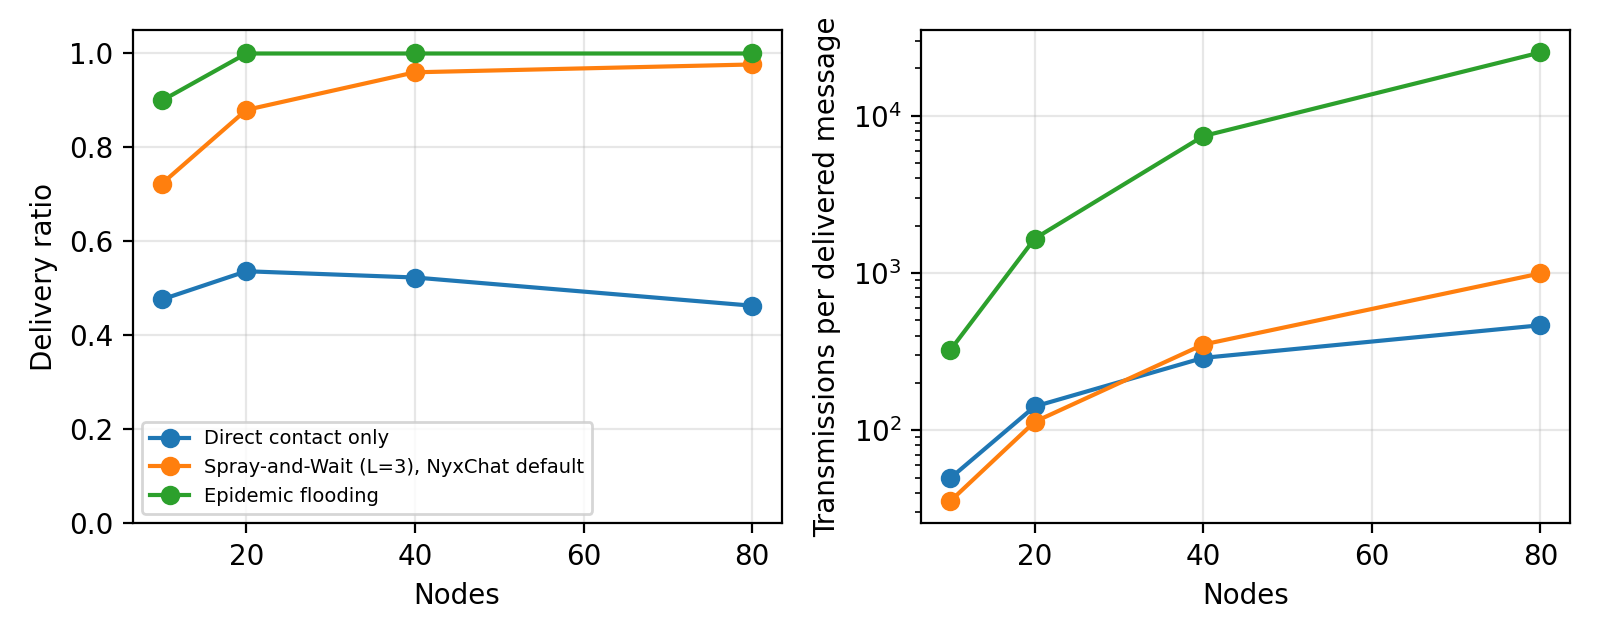
\includegraphics[width=\columnwidth]{figures/mesh_delivery.png}
\caption{Delivery ratio and transmission overhead versus node count for the three forwarding strategies.}\end{figure}
Direct contact delivers about half of the messages regardless of density, because delivery requires the two endpoints to meet within the run. Spray-and-Wait raises delivery to 72\% with 10 nodes and to 98\% with 80 nodes, and cuts latency as density grows, while its transmission count per delivered message stays between 3\% and 4\% of epidemic flooding at 40 and 80 nodes (351 versus 7,417 and 994 versus 25,237). Epidemic flooding reaches every destination at 20 nodes and above and has the lowest latency, but its cost grows super-linearly with density, which on Bluetooth translates directly into battery and channel occupancy. The bounded per-node store stays around 30 packets in the default configuration. These results support the choice of Spray-and-Wait with route learning as the default and quantify what a user gives up relative to flooding: at 20 nodes, 12\% of messages, which in the application are not lost but wait in the outbox for a later contact.

\subsection{7.4 Case study: the previous release}
Before this work the same application (version 2.0) advertised a Double Ratchet, hybrid post-quantum key exchange and a BLE mesh. Reviewing the code found the following:

\begin{itemize}
  \item The ratchet initialised both sending and receiving chains from the root key while the receiver performed a Diffie-Hellman step on the first message the sender had not performed, so the first message after any DH step failed to decrypt; the failure was caught and the raw ciphertext was displayed as the message text. Sessions were held only in memory and re-derived from static identity keys on every launch, providing no forward secrecy against identity-key compromise.
  \item Hello messages were unsigned and keys were never pinned; anyone on the network could claim any handle. All metadata travelled in cleartext over TCP.
  \item The Kyber library expects the module rank (3) where the code passed the security level (768), so every encapsulation threw an exception that was caught and logged, and every session silently fell back to classical keys.
  \item The Bluetooth library used was central-only; no device ever advertised the service UUID that the scanner filtered on, so two instances could not discover each other, and no code path sent a chat message over the mesh or consumed the router's delivery callback.
  \item Group messages used a static Diffie-Hellman key per pair with no forward secrecy; acknowledgements were received but never processed; the relay, Tor, privacy and stealth modules were not connected to anything.
\end{itemize}
None of these defects was visible from the documentation or the user interface, which showed lock icons and "encrypted" banners throughout. We draw two conclusions. First, security claims in this class of application must be backed by tests that exercise adversarial cases (tampering, replay, reordering) and by an honest threat model, which we provide with the source. Second, the mesh transport and the protocol must be designed together: our envelope abstraction exists precisely so that the same authenticated unit is used on every path and so that a transport cannot be "wired later".

\section{8. Security Analysis}
We argue informally for each goal of Section 3; a machine-checked model is future work.

\textbf{Confidentiality and integrity against observers and relays.} Message content and in-conversation metadata are inside envelopes encrypted under per-message keys that both parties derive from the ratchet, whose root comes either from the handshake master secret or from the asynchronous agreement. An observer or relay holds neither. The associated data binds sender, recipient and kind, and the ratchet header is authenticated, so modification or re-addressing is detected. Duplicates and replays are rejected because a consumed message key is deleted and a skipped-key entry is removed once used.

\textbf{Peer authentication.} After first contact, a peer must present the pinned identity key and prove possession of it: the handshake signature is over a transcript that includes the fresh nonces, and the master secret includes dh1, which an impostor without the identity private key cannot compute. On true first contact the design is trust-on-first-use, the same assumption Signal makes before safety-number verification; contact cards remove even that assumption.

\textbf{Forward secrecy and post-compromise security.} Every direct-link handshake contributes ephemeral values (dh2, dh3, dh4), so recorded sessions remain confidential after an identity-key compromise. Within a session the Double Ratchet deletes chain and message keys as it advances and heals after a compromise once the honest party performs a DH ratchet step \cite{ref2,ref3}. Asynchronous sessions are the weaker case: until the recipient replies, confidentiality against later compromise of the recipient's identity key rests on the sender's ephemeral key alone (dh2), exactly as in X3DH without one-time pre-keys; it is restored at the first reply.

\textbf{Post-quantum confidentiality.} The KEM secret enters the master secret and the asynchronous root through HKDF alongside the classical values. A quantum adversary that breaks X25519 still needs the Kyber decapsulation key; conversely, a flaw in the Kyber implementation leaves the classical security intact. We stress that \texttt{package:post\_quantum} is an unaudited implementation of the pre-standard Kyber construction; the hybrid combination is what justifies relying on it at all, and swapping in an ML-KEM binding changes one file.

\textbf{Link privacy.} A LAN observer sees the two hellos, which reveal handles, display names and public keys, and thereafter only sealed frames whose lengths and timing leak activity. Stealth mode suppresses the discovery announcements that would otherwise reveal presence even without a connection.

\textbf{Data at rest and coercion.} The database is unreadable without the master key, which is either keystore-protected or Argon2id-wrapped. The duress profile has its own keys and boxes, so the real identity and contacts are not exposed by opening it, and its optional wipe-first behaviour leaves nothing to recover. An adversary with a disk image is bounded by the password's entropy and the Argon2id cost, not by the in-app attempt counter.

\textbf{Residual risks.} Mesh addresses are stable hashes of handles, so colluding relays can learn that two hashed identities communicate and how often; a sealed-sender construction with rotating recipient tokens would remove this and is planned. Group membership is authenticated only to current members: a malicious member can add anyone. The application has not been formally verified or externally audited.

\section{9. Limitations and Future Work}
The Bluetooth transport has been exercised through the simulator and compiles for Android, but this paper does not report measurements from a physical multi-device deployment; throughput, connection stability across Android vendors, and battery cost under continuous scanning and advertising are the most important open questions and the subject of ongoing testing. Files require a direct link; chunked transfer over the mesh is possible but was excluded to protect relay storage. The simplified DHT and the internet relay exist in the code but are not part of the default path and lack NAT traversal and Sybil resistance. Legacy handles from version 2 are still accepted and are derived from only 32 bits of key material; they remain safe only because trust rests on pinned keys, and they will be retired. Planned work includes an iOS peripheral, an audited ML-KEM binding, sealed-sender mesh addressing, a formal model of the asynchronous initiation and collision rules, and a field study with volunteer users in a connectivity-constrained setting.

\section{10. Conclusion}
NyxChat shows that a messenger can be both infrastructure-free and cryptographically conservative. By making an authenticated, forward-secret envelope the only unit that any transport carries, the same guarantees hold over an encrypted Wi-Fi link, through a chain of untrusted Bluetooth relays, and across days spent in an outbox; by deriving sessions from pinned keys with a deterministic collision rule, asynchronous messaging works without a server; and by pinning keys and exposing safety numbers, users can detect the attacks that have broken earlier mesh messengers. The evaluation quantifies the cost of these choices, roughly half a kilobyte per message and tens of milliseconds per handshake, and the delivery achievable by bounded replication, 72-98\% across the densities studied at a small fraction of the cost of flooding. The case study of the previous release is a reminder that these properties exist only when the code, the tests and the documentation agree; all three are published with this paper.

\begin{thebibliography}{23}
\bibitem{ref1} M. Marlinspike and T. Perrin, "The X3DH Key Agreement Protocol," Signal Technical Specification, rev. 1, Nov. 2016.
\bibitem{ref2} T. Perrin and M. Marlinspike, "The Double Ratchet Algorithm," Signal Technical Specification, rev. 1, Nov. 2016.
\bibitem{ref3} K. Cohn-Gordon, C. Cremers, B. Dowling, L. Garratt, and D. Stebila, "A Formal Security Analysis of the Signal Messaging Protocol," Journal of Cryptology, vol. 33, pp. 1914-1983, 2020.
\bibitem{ref4} E. Kret and R. Schmidt, "The PQXDH Key Agreement Protocol," Signal Technical Specification, rev. 3, 2023.
\bibitem{ref5} National Institute of Standards and Technology, "Module-Lattice-Based Key-Encapsulation Mechanism Standard," FIPS 203, Aug. 2024.
\bibitem{ref6} M. R. Albrecht, J. Blasco, R. B. Jensen, and L. Marekova, "Mesh Messaging in Large-Scale Protests: Breaking Bridgefy," in Topics in Cryptology (CT-RSA), LNCS 12704, Springer, 2021, pp. 375-398.
\bibitem{ref7} M. R. Albrecht, R. B. Jensen, and L. Marekova, "Collective Information Security in Large-Scale Urban Protests: the Case of Hong Kong," in Proc. 30th USENIX Security Symposium, 2021, pp. 3363-3380.
\bibitem{ref8} T. Spyropoulos, K. Psounis, and C. S. Raghavendra, "Spray and Wait: An Efficient Routing Scheme for Intermittently Connected Mobile Networks," in Proc. ACM SIGCOMM Workshop on Delay-Tolerant Networking (WDTN), 2005, pp. 252-259.
\bibitem{ref9} A. Vahdat and D. Becker, "Epidemic Routing for Partially-Connected Ad Hoc Networks," Duke University, Tech. Rep. CS-200006, 2000.
\bibitem{ref10} K. Fall, "A Delay-Tolerant Network Architecture for Challenged Internets," in Proc. ACM SIGCOMM, 2003, pp. 27-34.
\bibitem{ref11} Briar Project, "Briar: Secure messaging, anywhere," and "Bramble Transport Protocol," https://briarproject.org, accessed Sept. 2026.
\bibitem{ref12} Meshtastic, "Meshtastic: An open source, off-grid, decentralized mesh network," https://meshtastic.org, accessed Sept. 2026.
\bibitem{ref13} WhatsApp, "WhatsApp Encryption Overview," Technical white paper, 2017 (updated 2023).
\bibitem{ref14} P. Rosler, C. Mainka, and J. Schwenk, "More is Less: On the End-to-End Security of Group Chats in Signal, WhatsApp, and Threema," in Proc. IEEE European Symposium on Security and Privacy (EuroS\&P), 2018, pp. 415-429.
\bibitem{ref15} A. Biryukov, D. Dinu, D. Khovratovich, and S. Josefsson, "Argon2 Memory-Hard Function for Password Hashing and Proof-of-Work Applications," RFC 9106, Sept. 2021.
\bibitem{ref16} H. Krawczyk and P. Eronen, "HMAC-based Extract-and-Expand Key Derivation Function (HKDF)," RFC 5869, May 2010.
\bibitem{ref17} A. Langley, M. Hamburg, and S. Turner, "Elliptic Curves for Security," RFC 7748, Jan. 2016.
\bibitem{ref18} Apple Security Engineering and Architecture, "iMessage with PQ3: The new state of the art in quantum-secure messaging at scale," Apple Security Research Blog, Feb. 2024.
\bibitem{ref19} Bluetooth SIG, "Bluetooth Core Specification, Version 5.0," Dec. 2016.
\bibitem{ref20} Berty Technologies, "Wesh Network Protocol," https://berty.tech, accessed Sept. 2026.
\bibitem{ref21} J. Bos, L. Ducas, E. Kiltz, T. Lepoint, V. Lyubashevsky, J. M. Schanck, P. Schwabe, G. Seiler, and D. Stehle, "CRYSTALS-Kyber: A CCA-Secure Module-Lattice-Based KEM," in Proc. IEEE EuroS\&P, 2018, pp. 353-367.
\bibitem{ref22} D. J. Bernstein, N. Duif, T. Lange, P. Schwabe, and B.-Y. Yang, "High-speed high-security signatures," Journal of Cryptographic Engineering, vol. 2, pp. 77-89, 2012.
\bibitem{ref23} N. Unger, S. Dechand, J. Bonneau, S. Fahl, H. Perl, I. Goldberg, and M. Smith, "SoK: Secure Messaging," in Proc. IEEE Symposium on Security and Privacy, 2015, pp. 232-249.
\end{thebibliography}
\end{document}
